\documentclass[lof,lot,12pt]{puseniorthesis}
% options to class:
% lof, lot, lost - generate list of figures, tables, symbols
% filecopy, advisercopy, readercopy - note that this is 'File Copy', 'Adviser Copy', 'Reader Copy' on title page

\usepackage{xcolor}
\usepackage{graphicx} % needed for \includegraphics
\usepackage{amsmath}
\usepackage{float}
\usepackage{todonotes}
\usepackage{hyperref} % used for hyperlinked, verbose references
\usepackage{cleveref}
\usepackage{subfigure}

%%
%% REQUIRED INPUTS
%%
\author{Katherine Denner}
\classyear{`19}
\adviser{Daniel Steingart}
\reader{Craig Arnold}
\title{Identification of lithium deposition and characterization of state of charge and health in extreme fast charge cells using ultrasonic methods}
\dept{Mechanical and Aerospace Engineering}
\submitdate{01 May 2019}
\course{MAE442}
\abstract{%%
%% MOTIVATION
%%
High performance batteries such as those critical to electrical vehicle adoption require constant, accurate estimation of many cells' state of charge and state of health, and deft management of the battery based on that information is critical both to vehicle performance and safety. 
Inadequacies in the state of the art are holding back more widespread electric vehicle adoption. 

This thesis builds on prior work in developing new, ultrasonic methods for measuring battery state of charge and state of health in operando, and for the first time demonstrates the technology's ability to measure ambient temperature, a key metric for both performance and safety in electric vehicles.
Prior work in this area targeted standard consumer battery formats such as AA. 
The fast-charge batteries favored by high-performance applications such as electric vehicles present additional challenges due to their more rapidly-shifting properties and more compact form factors, yet also present greater opportunity because so much more can be gained by improving their performance. 
The work herein focuses on extreme fast-charge cells, but its results can be generalized to other cells which are easier to work with.

Described within is the design of an experimental apparatus was designed tp allow for electrically manipulating the lithium-ion cell's state of charge and state of health while regulating its ambient temperature and pressure; the experimental procedures used to explore the validity of these acoustic time of flight techniques to lithium-ion fast-charge cells; and the data analysis used to synthesize and interpret acoustical, electrochemical, and thermal data.

Ultimately, this thesis demonstrates the capability of acoustic time of flight analysis to observe changes in the state of charge and state of health in a fast-charge lithium-ion cell, and for the first time, to observe changes in the cell's ambient temperature.}

%%
%% OPTIONAL INPUTS: NOTES, DEDICATION, ACKNOWLEDGEMENTS
%%

%\extranotes{These are a few lines of optional notes} 
%\dedication{To}
\acknowledgements{
I thank Clem, Wes, Tom, and particularly Greg for their patience and support.
\\
This would not have been possible without Glenn and Al. Sorry about the CNC.
\\
I am grateful for funding from the John Marshall II Memorial Prize Fund.
}

\numberwithin{equation}{section}

%%
%% CONTENT: CHAPTERS, BIBLIOGRAPHY, APPENDICES
%%
\begin{document}

\chapter{Introduction}

\section{Motivation}
Increasing demand for electric vehicles is pushing the need for extreme fast charge capabilities in lithium battery chemistries, and a critical limiting factor in charging rates is lithium deposition \cite{XFC}. Charging a lithium battery too quickly causes lithium deposition, which reduces cell capacity and in severe cases, creates safety hazards \cite{XFC}. Currently there is no practical in operando method of detecting lithium deposition. Without real-time lithium deposition monitoring, safety and financial considerations require batteries with lithium-based cells to use controllers programmed to charge and discharge conservatively. Being able to monitor lithium plating would allow battery management systems for lithium cells to more accurately control charging rates, and potentially even employ charge and discharge protocols that unplate lithium.

The objective of this thesis is to use ultrasonic methods to demonstrate the feasibility of detecting the deposition of lithium and determining changes in the state of charge and state of health of single layer, high-rate lithium ion cells.

%% broad introduction
% when choosing what to include, assume the reader will only skip it
%   include any critical background in a subsection of the relevant chapter
\chapter{Background}

\section{Lithium Ion Fast Charge Cells}

\subsection{Lithium Ion Battery Chemistry}
Increasing demands on the energy density and form factor of rechargeable batteries created a massive and growing market for lithium ion battery cells \cite{LBST}. 
Their superior gravimetric and volumetric energy densities are due to the high cell voltages (~4V), which are made possible by the non-aqueous electrolytes of lithium cells \cite{LBST}. Batteries work by passing ions back and forth between two electrodes - separated, charged materials. In its fully charged state, a battery cells charge has collected on its negatively-charged electrode (the anode). 
The ions are keen to flow to a lower energy state, and flow readily to the positively charged electrode (the cathode), shedding their electrons to the circuit in the process and powering the connected device. 
As more of the ions jump to the cathode, the energy imbalance between the two plates shrinks, until charged particles are no longer easily motivated to move from the anode to the cathode. 
In a rechargeable battery, this process is reversible, and if electrons are fed back to the cathode by reversing the circuit, ions will flow back to the anode \cite{ LBST}. In a lithium ion battery, these ions are Li$^+$. \todo{get cell chem}.

The voltage of a battery is simply its potential energy per charge, and the open-circuit voltage $V_{oc}$ of a lithium-ion cell is a function of
$$ V_{oc} = \frac{\mu _{Li(c)} - \mu _{Li(a)}}{F} $$
where $\mu_{Li(c)}$ is the lithium chemical potential of the cathode, $\mu_{Li(a)}$ is the lithium potential of the anode, and $F$ is Faraday's constant (the charge in Coulombs of one mole of electrons) \cite{LBST}.
Good charge and discharge performance requires that the "lithium insertion/extraction process should be reversible with no or minimal changes in the host structure over the entire range $x$ of lithium insertion in order to provide a good cycle life for the cell" \cite{LBST}.

\subsection{Lithium Plating}

\subsection{Charging Protocols}

stage 0: preconditioning

If the cell was deeply discharged, it should first be charged at a very low current, so that minimal heat is generated before the cell is in such a state that it can deal with that heat \cite{DIGIKEY}.

stage 1: constant-current 

Drive the cell at a constant current to get its voltage to 4.2V. The higher the current, the faster this charging stage happens, but also the more damage delivered to the cell \cite{TI}. Charging rates are often limited to 1C, but fast charging can allow for higher rates \cite{TI}.

stage 2: constant-voltage 

Charge with constant-voltage until the current steps down to ~0.1 Amps, at which point charging is complete \cite{DIGIKEY}. Constant-voltage charging prevents overcharge \cite{DIGIKEY}. The decreasing current required to maintain 4.2V is what creates the exponential decay shape of the current vs time plots during charging \cite{TI}.

\subsection{Charging Rates}
To normalize across battery capacities, charge or discharge current is often expressed as a C-rate \cite{SPECS}. A C-rate expresses the rate a battery at which a battery is discharged in terms of its maximum capacity; a 1C rate will fully discharge a battery in 1 hour, a C/2 rate will do so in 2 hours, and a 2C rate will discharge a battery in 1/2 hour \cite{SPECS}. Since the cells being investigated in this work have a roughly x Amp-hours \todo{number} capacity, a 1C rate uses \todo{number} Amps for charging, whereas a 10C rate uses \todo{number} Amps.

\section{Acoustic Time of Flight (ToF) Analysis}
Recent work has shown that Acoustic Time of Flight (ToF) Analysis can show the state of charge and state of health of battery cells.

Acoustic ToF analysis probes a unit with continuous acoustic waves, and makes conclusions based on how long it takes for waves to travel to the receiver (either the waves which travel through the test unit to a receiver, or the waves which reflect off of the material and back to the transmitter). How long it takes for a wave to travel from one point to another depends on the ubiquitous relation 
$$\text{distance} = \text{ rate} \times \text{ time} \rightarrow \text{ time} = \frac{\text{distance}}{\text{rate}}$$

Nondestructive ultrasonic analysis measures the time of flight (how long it takes the wave to travel either back to the transmitter, or to a receiver), and the amplitude of the received signal. These quantities can be used to estimate the thickness of the material, $T$:
$$ T = \frac{ct}{2}$$

where $c$ is the material sound velocity, an $t$ is the duration of the flight \cite{OLYMPUS}. 
Thus, if $c$ can be assumed constant, $T$ can be measured using only $t$.
Ensuring $c$ can be assumed sufficiently constant was an important consideration in apparatus design, to be discussed later.

High frequency waves are used because BLANK however BLANK

\subsection{Prior Work}

Hsieh et al \todo{cite?} performed electrochemical-acoustic time-of-flight (EAToF) experiments on batteries of various chemistries and form factors, demonstrating "strong correlation between SOC and the density distribution within a cell, as determined by acoustic measurements" \cite{TOF-STATE}. They go on to conclude that "changes in the ToF echo profiles and acoustic signal amplitudes as a function of cycle number appear to be key indicators of central phenomena occurring within the battery, including changes in intraparticle and interparticle stress and strain, as well as the formation and removal of critical surface layers", suggesting but not demonstrating that electrochemical-acoustic ToF analysis can determine a battery cell's state of health.

That assertion was demonstrated in the subsequent paper by Bhadra et al \todo{cite?} \cite{ANODE-CHAR}, which demonstrated the capacity of electrochemical acoustic time-of-flight analysis to "examine the dynamic properties of cells during discharge" "by tracking the saturation of the central echo and secondary echos, the total shift in the ToF peak position over discharge, and total transmitted signal amplitude".

This work was built on by Davies et al \todo{cite?} \cite{SOC-SOH-EST}, who explored the accuracy of the EAToF method while cycling lithium-ion pouch cells over hundreds of cycles, focusing on "two key metrics: time of flight shift and total signal amplitude, which are the used with voltage data in a supervised machine learning technique to build a model for the state of charge (SOC) prediction". 
In addition to showing their model was about $99\%$ accurate for two different cell chemistries, they showed that the model can be extended to predict state of health with similar accuracy by adding to the model the full ultrasonic waveforms at top of charge.

\todo{Other factors which affect $c$}
What some noise contributions are % \input is a lower-level \include that is typically slower but allows nesting

%input{literature}

%\input{subject} % include pulls from precompiled .aux and is faster than \input, but won't work with labels from other sections; use it when able

\chapter{Apparatus design}

\section{Considerations}
\begin{enumerate}
    \item Frequency: resolution vs attenuation
    \begin{enumerate}
        \item Thinner cells require shorter wave lengths for useful resolution
	    \item Shorter wavelengths require higher frequencies
		\item Higher frequencies introduce greater attenuation
	\end{enumerate}
	\item Set-up: avoid near-field effects without introducing significant impedance
		\begin{enumerate} 
		    \item impedance is the result of medium transitions (e.g. the light traveling through air into a pool of water problem from physics)'
		    \item The near-field effects make the earliest readings highly unwieldy
	        \item Need to develop an apparatus that places enough distance between the transducer and the cell that the near-field effects have fallen away, but does so without introducing significant new impedances - be sure to impedance match materials and minimize number of materials
	    \end{enumerate}
	\item Pressure vs performance
	    \begin{enumerate}
		\item Need to exert enough pressure on the cell to ensure quality, consistent readings, but not so much that it materially effects battery behavior
		\item Should be adjustable
		\item Should apply a consistent pressure (<=0.5MPa) for SOC/SOH reasons, preferably light (to reduce experiment rest times) but potentially heavy if additional lithium deposition needs to be forced (see Cannarella)
		\end{enumerate}
    \item Securely and planarly mount as many as three transducers (to compare readings from different regions of cell - deposition should be asymmetric since leads are on one side)
    \item Avoid clamping to the edges: the lamination sometimes causes lil bulges
\end{enumerate}

\section{Sensors}

\section{Structure}
The structure has the following goals:
\begin{enumerate}
    \item Secure cell unit under test (UUT)
    \item Locate cell UUT with some modicum of repeatability
    \item Secure the transducers in place
    \item Align the transducers perpendicular to the cell
    \item Separate the cell and the transducers sufficiently to reduce noise
\end{enumerate}

The basic apparatus is two similar clamps, each of two blocks of aluminum which bolt together. Aluminum was chosen for its strength and machinability. The largest block has all the mounting holes for bolting the plastic transfer medium to the clamp, and for bolting the clamp to the rail. The second piece is much smaller, used only for securing the transducers; it had to be seperated from the main body of the clamp due to the form factor of the transducer. This section is sandwiched tightly in place between the main body of the clamp and the plastic transfer media. The block of plastic acts as a transmission medium for the ultrasonic waves to move between the transducers and the cell. The second block has a series of holes for holding the transducers. The total apparatus has two of these clamps, one of which is bolted directly to the rail and stays stationary, and the other of which is bolted to the carriage and is actuated to secure and release the cell for testing.

To actuate the clamps, one of the clamps is mounted to a carriage which rides along a rail. A piston (controlled by a Pithy microcontroller) actuates to push the clamp into place to secure the cell, or pulls the clamp away to release the cell. The second clamp is rigidly bolted directly to the rail. This set-up allows the clamp to easily hold and remove the cell without adding unnecessary degrees of freedom. To locate the cell unit under test, the smaller block of the clamp fits around the cell, using the tabs for the leads as rough locators.

Holes are cut into the clamp for the transducers to sit in. Below those holes are a second set of holes, smaller in diameter, for springs. The springs push the transducers flush against the transfer medium. They are tensioned by bolting the two halves of the clamp together, forcing the transducers into alignment with each other and with the cell. The transducer cables pass through clots cut into the side of the block.

The second block in the clamp, the plate, is merely for holding the plastic which acts as transfer medium. Its purpose is to ensure that the ultrasonic waves experience Fraunhofer (far field) diffraction, rather than noisy Fresnel (near field) diffraction. \todo{do I need to cite this section?}
Fraunhofer diffraction occurs when
$$ \frac{W^2}{L\lambda} << 1$$
where $W$ is the aperture or slit size, $L$ is the distance from the aperature, and $\lambda$ is the wavelength.
$\lambda$ needs to be minimized for this experiment (thinner cells require shorter wavelengths for useful resolution of data, and $W$ is a variable we would rather not shrink below the diameter of the transducers in order to avoid interfereing with the transducers' data collection, which leaves only $L$ available for manipulation. Introducing a distance between the transducers and cell allows the experimental set-up to avoid Fresnel diffraction, but also introduces some losses due to the change in transmission media \todo{be more specific here}. The magnitude of the losses depends in part on the difference in the impedances of the two media, so \todo{material} was selected for its similar impedance to \todo{cell material} and its machinability. Machinability is important \todo{because}.
 
\section{Actuator}
Pneumatic piston was chosen for:
\begin{enumerate}
    \item relatively low cost (since air infrastructure is already present in lab)
    \item low expected set-up/calibration time
    \item relatively high precision
    \item easily controlled by controlling the pressure of its intake
    \item doesn't introduce any unnecessary degrees of freedom
\end{enumerate}

Piston selection:
\begin{enumerate}
    \item Form factor: flat sides, lots of mounting holes to conveniently and securely mount to structure
    \item Force output: Will most probably want to exert a pressure in the range of 0-0.5 MPa (Cannarella's "low stack pressure"), but want to leave the option open of exerting a stack pressure of 1.5-3.0 MPa on cell (Cannarella's "high stack pressure"), in order to induce lithium plating if necessary; if this is done across an area of ~20cm\^2. McMaster (a convenient supplier) offers pistons of the desired form factor with force ratings of up to 779lbf at 100 psi, which assuming a clamp area of 4.5 cm\^2, would result in an exerted stack pressure of about 1.7 MPa.
    \item Double-acting: will allow the piston to both push and pull itself, allowing for a more automated set-up
\end{enumerate}
     % use input rather than include so that labels sync

% lithium ion: lithium cobalt oxide / graphite
% 0.30 mAh
\chapter{Experimental Procedure}
The goal of the first experiment was to force plating via electrochemical cycling, and acoustically observe this in the moment using ToF data. It was unsuccessful due to overwhelming noise due to uncontrolled ambient conditions. In response, several improvements were made to the experimental apparatus in an attempt to eliminate appreciable noise in the ToF data due to ambient conditions. The second experiment's goal was to determine whether these changes adequately controlled the ambient conditions to prevent them from overwhelming the ToF data with noise; it was successful. The experiment showed a close and consistent relationship between time of flight and cell state of charge (ToF and SoC).

Recall that thre three main determinants of change in acoustic wave time of flight through a battery cell are thought to be ambient conditions (most relevantly, temperature and pressure), state of charge, and state of health. Now that the set-up was validated to have minimal change in ambient conditions, and a relationship between ToF and SoC strongly established, further experimentation could reasonably explore the relationship between the cell's state of health and acoustic time of flight. The goal of the third experiment was to force plating via purposefully reckless electrochemical cycling, and acoustically observe this while it happens using ToF data; it was successful. The goal of the fourth experiment was to establish how reckless cycling would need to be in order to induce plating, by cycling at 5C but never 10C rates of charge; the 5C charge cycles were found to induce little plating \todo{discuss temps}. The goal of the fifth experiment was then to induce just some plating in the cell, by loading at a 10C charge rate for only one charging cycle; it was successful. Then, the goal of the sixth experiment was to establish a baseline for the ToF data without any plating by repeatedly (20 times) loading a cell at a very low rate of charge (C/2.5) to better understand the acoustic ToF response when no appreciable plating occurs.

\section{Observing ToF Shifts Due to State of Charge}

\subsection{Acoustic Monitoring of Cell Cycling in Unsteady Conditions}

The cell was cycled (charged and discharged) five times at a C/2.5 rate. 
Both the battery cell and the transducers used to send and receive the acoustic waves are subject to changes in operating characteristics due to change in temperature, so each testing protocol begins with a long rest to give the unit under test and the testing equipment time to acclimate to the ambient conditions. 
Then, the cell charges at a constant-current rate of 0.0120 Amps. 
The C/2.5 rate was chosen because such a gentle rate would induce very little lithium plating, and state of health of the cell would be roughly constant. 
If the cell's state of health did not change between cycles, and the experiment's ambient conditions held steady, then all changes in acoustic time of flight can be assumed to be due to change in state of charge.
The cycle then rested ten minutes, was discharged using the same constant-current, 1/2C protocol, and then rested for ten minutes again. 
The rests between and within cycles allow for the cell to reach new steady-state conditions. 
There was a potential for the cell to experience somewhat significant transient effects due to phenomena such as the heat addition or structural stiffening during the oxidation-reduction reaction of cyclic charging and discharging; the rest cycles give the cell time to relax and modulate.
Then, the rest-charge-rest-discharge sequence was repeated for a total of five cycles.

\todo{insert flowchart}

Unfortunately, the assumption that the ambient conditions were steady did not hold, leading to considerable noise in the in the readings due to environmental interference, ultimately drowning the acoustic ToF signal. At that point, the exact source of the noise was unknown.

\todo{insert plots?}
    
\subsection{Acoustic Monitoring of Cell at Rest in Unsteady Conditions}\label{chamberTest}
Since it was impossible to determine the source of changes in ToF data for the prior test, or to determine what was signal and what was noise, a more piecewise approach to building up the experiment was needed. Due to the very small size of the cell, small variations in temperature and pressure could theoretically have relatively large impacts on the speed with which high-frequency acoustic waves travel through the cell. Some possible solutions were identified as: regulating the temperature to be relatively constant, better regulating the pressure applied to the cell, and using higher frequency transducers to probe the cell. Switching the 2.5MHz transducers for 15MHz transducers was quick and easy since the second set of transducers was already on hand, so this was done for the next trial. Additionally, the relatively loosely fluctuating ambient temperature was expected to have a relatively large effect on time of flight, so the pressurizing apparatus was inserted into a thermal chamber, as described in \hyperref[thermalChamber]{\cref{thermalChamber}}. The stack pressure is already expected to be constant to within \todo{insert estimate}, so this was left unchanged, to be revisited only if necessary.

Additionally, the cycling was postponed to a later experiment.
For now, the cell would be left at rest for the duration of the experiment. 
If there was no significant shift in acoustic ToF data while the cell waited at rest for a long period, then the noise in the environment is adequately controlled and cycling experimentation can proceed. 
If there were still shifts, the environment would need further control, probably through higher-precision active temperature control and pressure control. 
Currently, the temperature is controlled only passively through thermal isolation, with the active temperature control having a pretty loose accuracy of about 1 degree \todo{verify}.
For 24 hours, the cell was probed ultrasonically while pressurized in the thermal chamber \todo{thermal, pressure data}.

\todo{plots}
The data show that the ToF did not shift while the temperature was held constant, and then shifted in step with a shift in temperature at the end, verifying that this setup effectively reduced environmental noise to acceptable levels to begin attempting to observe ToF shifts due to cell state.
\todo{describe plots}


\subsection{Acoustic Monitoring of Cell Cycling in Steady Conditions}
\todo{plots?}
Once the noise levels were brought under control, attempting to observe change of state via acoustic ToF shift could begin. The cycle was set up as in the first experiment, with a long initial rest period to ensure starting conditions were steady state, then five cycles of a 10 minute rest $\rightarrow$ 1/2C current-controlled charge $\rightarrow$ 10 minute rest $\rightarrow$ 1/2C current-controlled discharge; see \todo{fig}. 
\todo{discuss temps}
The system was kept pressurized to 2.4 PSI, which was a stack pressure of about 0.42MPa, falling into Cannarella's low stack pressure regime.

\section{Observing ToF Shifts Due to State of Health} 
Once confirmed that the experimental set-up was capable of observing change of state of charge of the cell, it could be investigated whether it could observe changes in state of health.

\subsection{Acoustic Monitoring of Lithium Plating}
\todo{flowchart}
The battery was set-up in the pressurized, thermally-regulated apparatus as before; this time at a temperature of \todo{temp} C and a system pressurization of \todo{pres} psi, which applied a stack pressure of \todo{stack}. 
The cell was again cycled but this time with aggressive ramps in charging rate. 
This intentionally reckless operation would force significant lithium plating to develop on the anode. 
After a rest to ensure steady-state conditions, the cell was given a ten minutes rest, charged at a 1C rate for 60 minutes, given 10 minutes rest, and discharged at a C/2 rate. 
This sequence was repeated once, for two total cycles. 
It was then repeated with a charging protocol of 2C for 30 minutes, then 5C for 12 minutes, then 10C for 6 minutes. 
Lithium plating was expected to be observed in the latter two cycles.
\todo{plots?}
    
\subsubsection{X-Ray Photoelectron Spectroscopy Analysis of Cell}
    To independently determine the extent of lithium plating in the cell, it was analyzed via X-Ray Photoelectron Spectroscopy.

\subsection{Acoustic Monitoring of Lithium Unplating}

\subsubsection{XPS Analysis of Cell}

\subsubsection{SEM Analysis of Cell}

\section{Observing ToF Shifts Due to Unsteady Conditions}

\subsection{Acoustic Monitoring of Rapidly Cycling Cell in Unsteady Conditions}

\section{Baseline Correlation Between TOF shifts and Acoustic Plating}
??

\chapter{Results}

The data clearly show first a relationship between cell state of charge the acoustic TOF through the cell, then between induced lithium plating and changes in acoustic time of flight data, and finally between changes in ambient temperature and change in acoustic TOF through the cell. 

Recall that the three sources of change in acoustic time of flight through a cell are change in state of charge, change in state of health, and change in ambient conditions. 
By systematically adding and understanding changes in each category to the experimental conditions, shifts in acoustic ToF through the cell can be observed, analyzed, and then attributed to each source of change.

When the ambient conditions were steady, the relationship between SoC and ToF was very clear \todo{plot}. Ambient temperature variation clearly has a significant effect on the acoustic TOF shifts. \todo{fig} shows a comparison between the measured TOF data and "idealized" TOF from a gentle, non-plating routine, constructed by assuming the data ought not change between cycles and copying the first waveform repeatedly as a result. In the absence of plating and at the same state of charge, the relationship between change in ToF shift and change in ambient temperature is consistent enough that much of the influence of temperature can be scrubbed out using simple regressions.

\section{Time of Flight Shift Due to Change in State of Charge}
The data clearly demonstrate a strong and consistent relationship between acoustic ToF through the cell and the cell's state of charge while ambient conditions and cell state of health are held steady.

The shift in ToF was determined using a colleague's cross-correlation analysis of each received waveform to a reference waveform. The reference waveform was chosen from one of earliest waveforms in the experiment, but not too early, in order to allow for start-up effects to dissipate.
During the C/2.5 charge and discharge cycling, which does not appreciably plate the cell and therefore can be assumed to not change the state of health of the cell, the ToF data follows a very regular pattern. 
The ToF shift peaks at roughly the same value, and at the same point in the cycling protocol: when the routine finishes charging. 
Conversely, the ToF shift experiences a minimum of fairly consistent value at the end of each discharge period.

\todo{fig}

\section{Time of Flight Shift Due to Change in State of Health}
The data in the same test goes on to demonstrate acoustic TOF analysis's capability to observe plating, and therefore change in a cell's state of health. This is shown during the 5C and especially 10C routines in the experiment. 
While the TOF data maintains a consistent form for each of those protocols, the "neutral axis" to which it returns between cycles increases each time. 
Since the ambient conditions were steady and there was no variation in the cycling protocols, these changes in the TOF shift show lingering changes in the state of health of the cell. 
This is corroborated in each of the experiments. 
SEM (scanning electron microscope) and XPS (X-Ray Photoelectron Spectroscopy) analysis confirm plating on the electrodes of the cells, but such techniques do not provide information on when the plating occurred. \todo{moar}

To confirm plating had indeed occurred, a cell was dissected and used for optical, SEM, and XPS analysis.

\begin{figure}[t]\label{fig:optical}
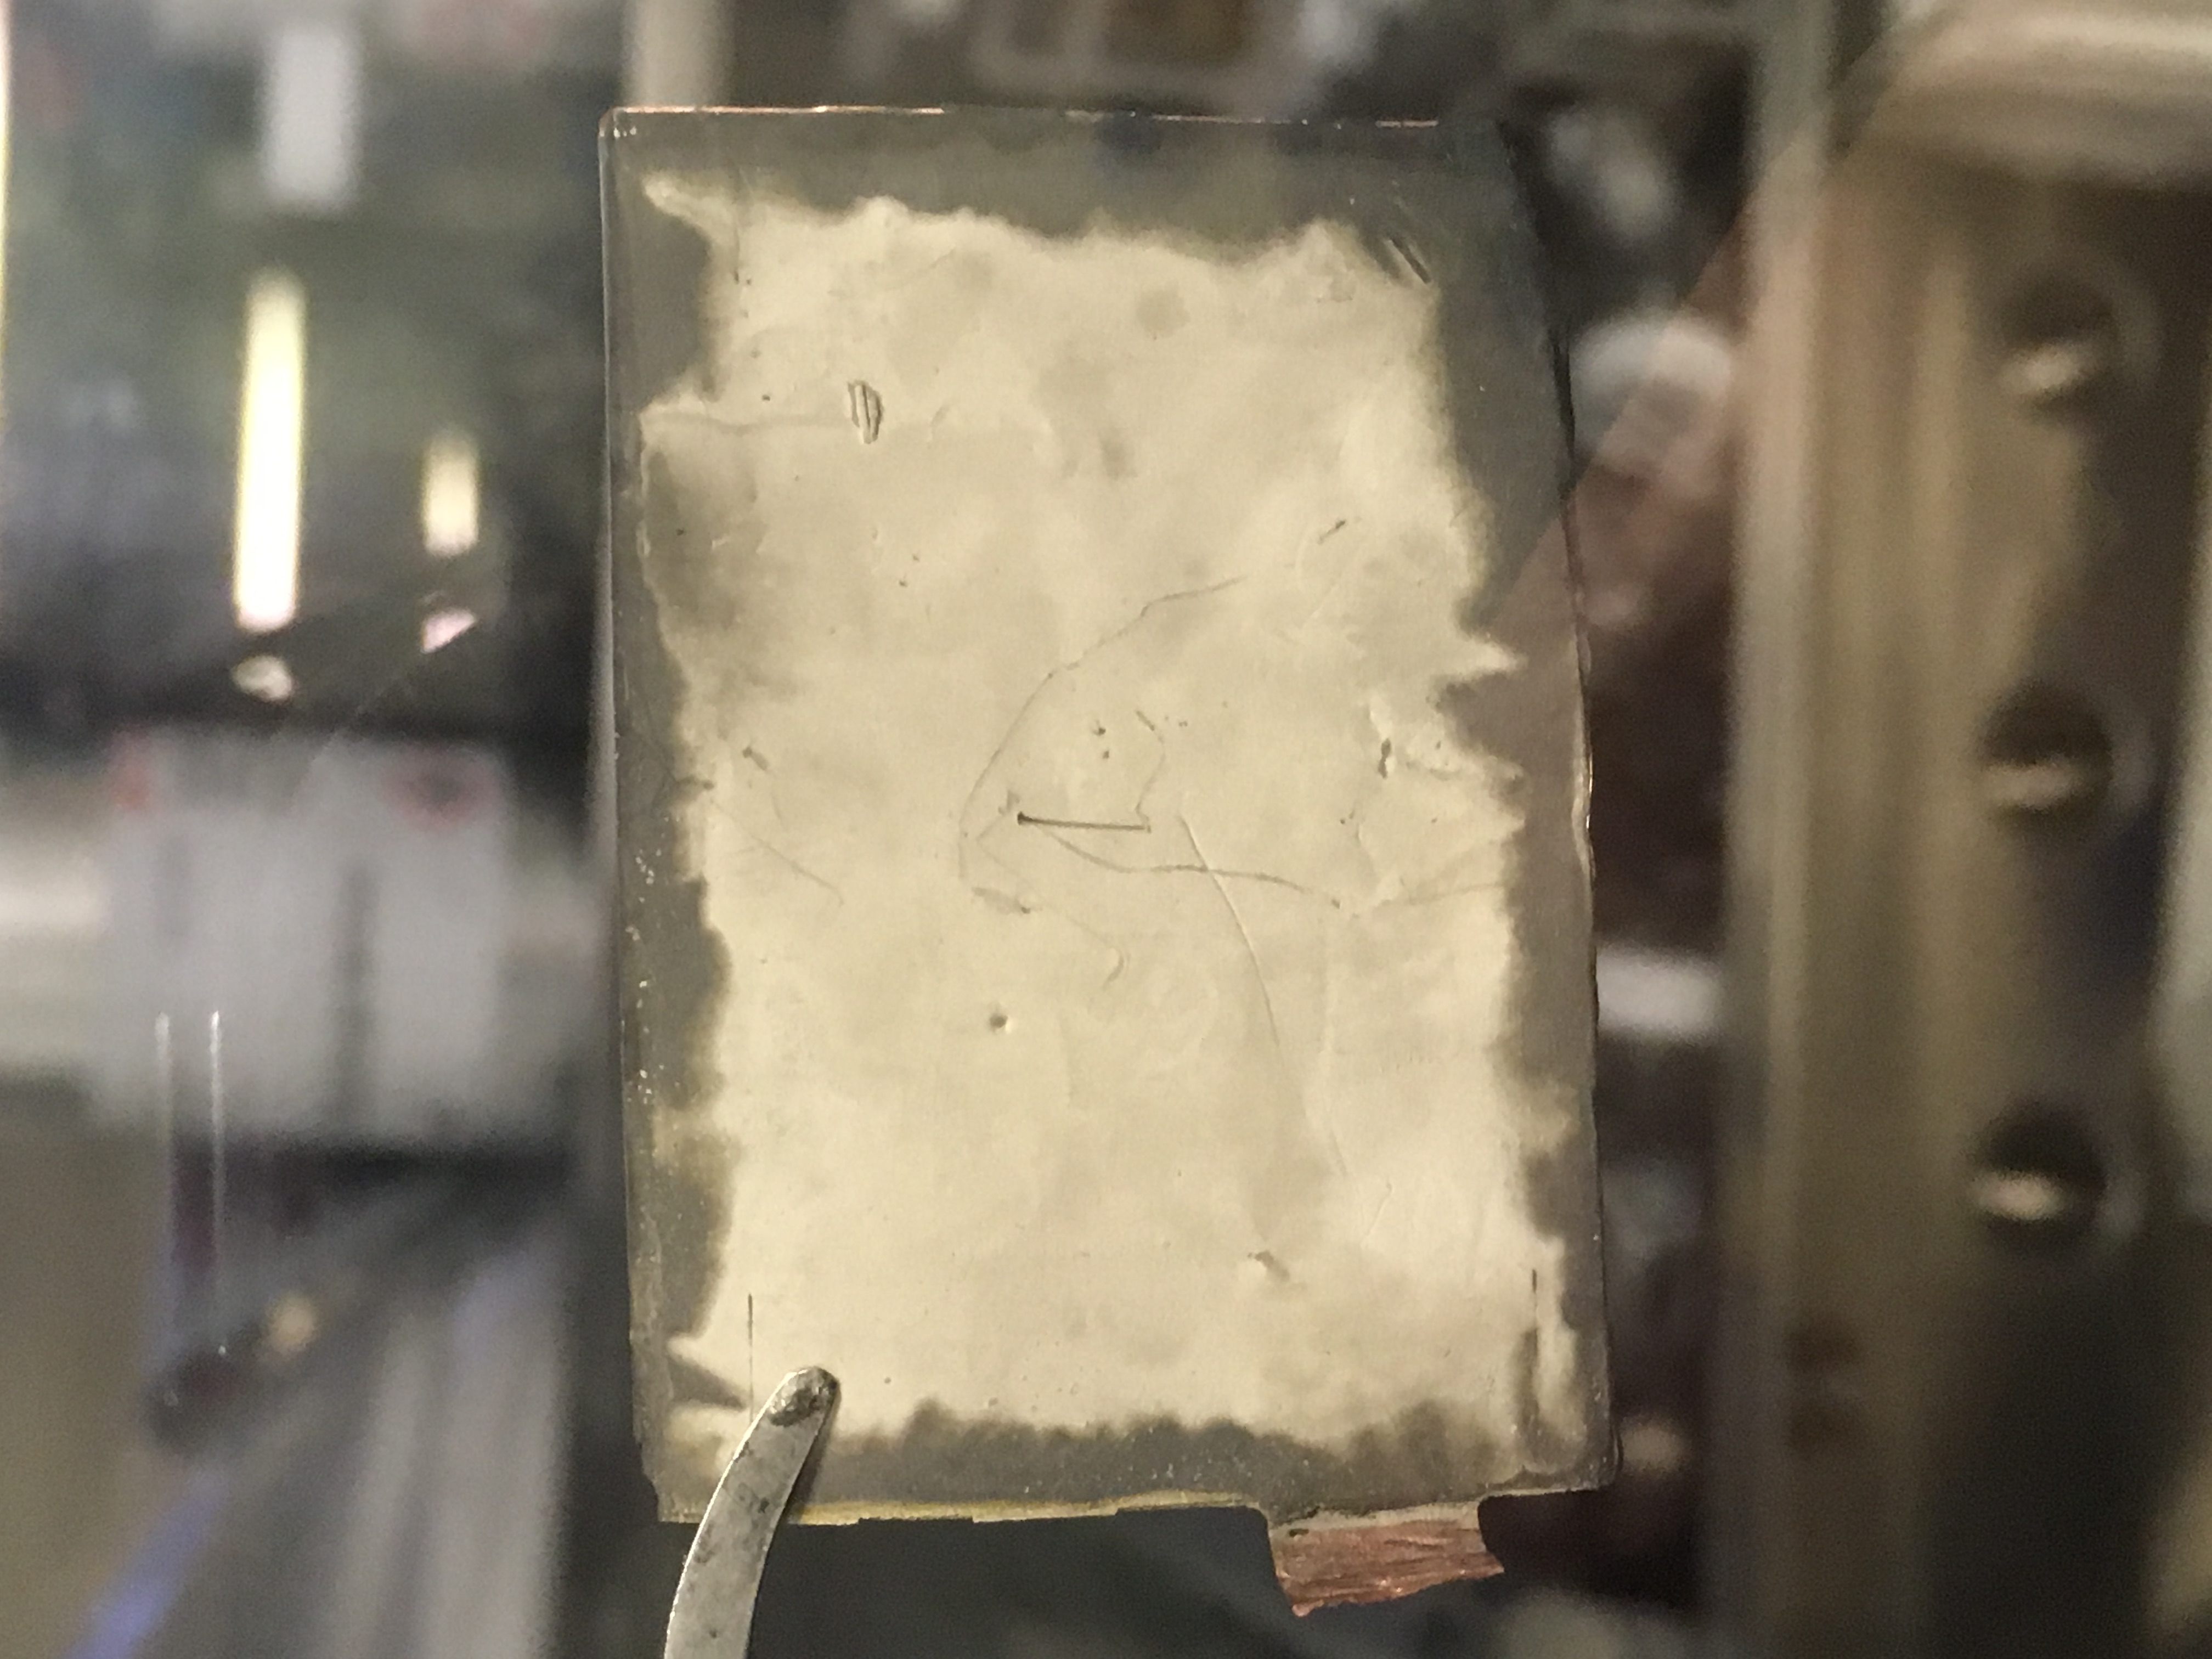
\includegraphics[width=0.6\textwidth]{Thesis/optical.JPG}
\centering
\caption{A cell cut open after electrochemical cycling. The light region is lithiated.}
\end{figure}

Optical analysis provided quick confirmation that the cell had plated; since the cell had not been used before the experimental protocol described above, it can be safely assumed the plating occurred then. SEM and XPS analyses provide more sophisticated information about the plating. 

\section{Time of Flight Shift Due to Change in Ambient Conditions}
In the first experiment which demonstrated the technique, ambient temperature was held quite steady, and had no material impact on acoustic TOF through the cell. 
However, subsequent experiments were unable to maintain such optimal conditions.
During routines using gentle C/2.5 cycling, thus maintaining state of health, the influence of ambient temperature changes on acoustic TOF can be isolated from the influence of state of charge changes with reasonable success. 
Polynomial fits and linear regressions correlate change in ambient temperature with change in ToF shift. 

The thermocouples and transducers have different sampling rates and schedules, so a couple approaches created paired change in ToF shift and change in temperature data; these are plotted against each other in \todo{ref}. 
In one version of the analysis, change in temperature data was averaged across a cycle and regressed against change in TOF shift data. 
More accurate results resulted from interpolating the temperature data using linear or polynomial fits, depending on the shape of the temperature data.

The analysis shows a reasonable estimate at how the ToF would shift without the influence of the ambient temperature shifts, potentially broadening the application of the technique in monitoring cells.
\begin{figure}[t]\label{fig:0417tofshiftadj}
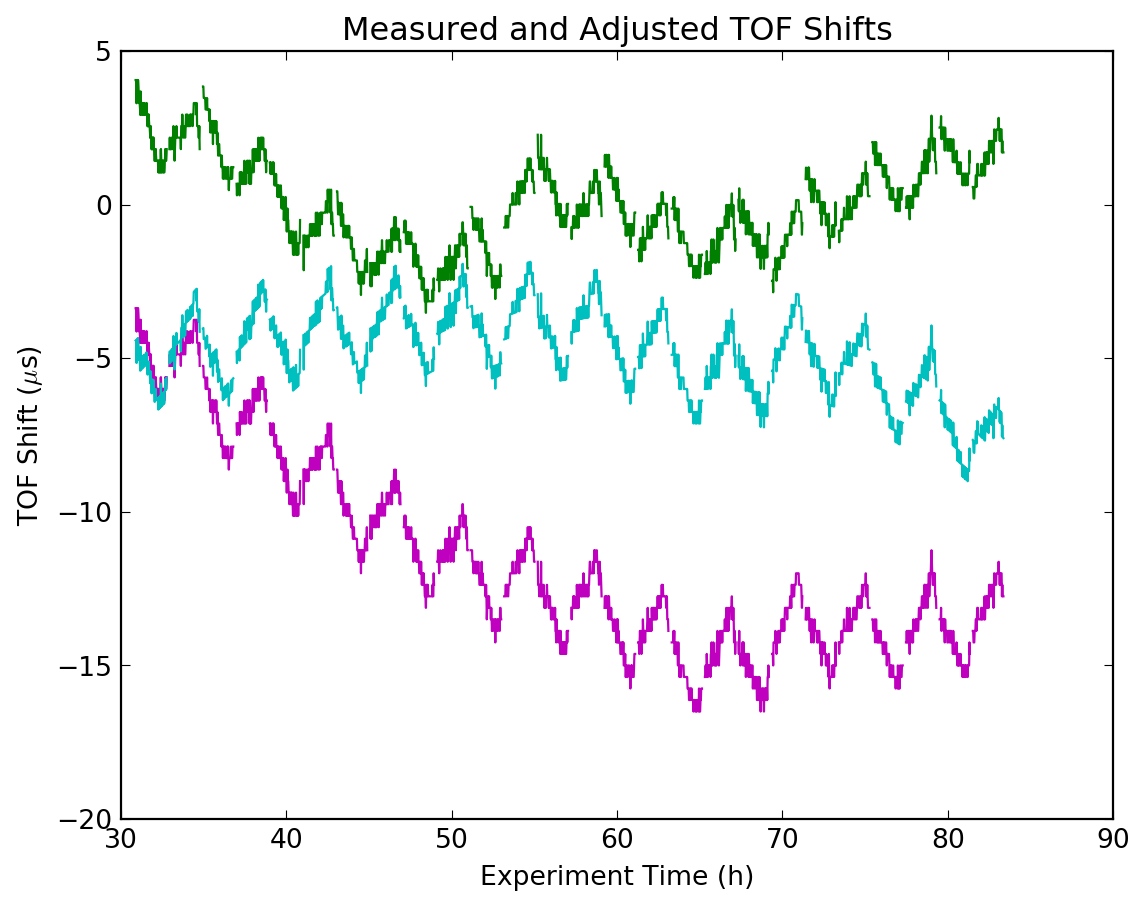
\includegraphics[width=0.75\textwidth]{Thesis/0417tofshiftadj.png}
\centering
\caption{ToF Shift across the experiment. This plot compares the unaltered ToF shift, the ToF shift adjusted using a change in ToF - change in temperature regression using interpolated temperatures, and the ToF shift adjusted using a regression of maximum change in ToF shifts and averaged temperatures.}
\end{figure}

One check is to compare them to an idealized prediction of how the TOF should actually shift during the experiment. 
Since each cycle at a particular charge rate has a consistent duration and consistent effect on the cell's state of charge, it is easy to compare ToF shift data between cycles. 
At any particular point in the cycle's duration, the ToF shift in each cycle should match. Charge and discharge cycle ToF data, when overlaid (see \hyperref[fig:0417overlays]{\cref{fig:0417overlays}}), show how consistent or inconsistent the ToF shifts are across the experiment.
Ideally there would be perfect overlap in the data from each cycle within a protocol within an experiment, but before the ambient temperature shift's influence was removed, this was clearly not the case. 
The overlap is still imperfect after the TOF shift data was adjusted based on the regressions, but it is much better.

\begin{figure}[t]\label{fig:0417overlays}
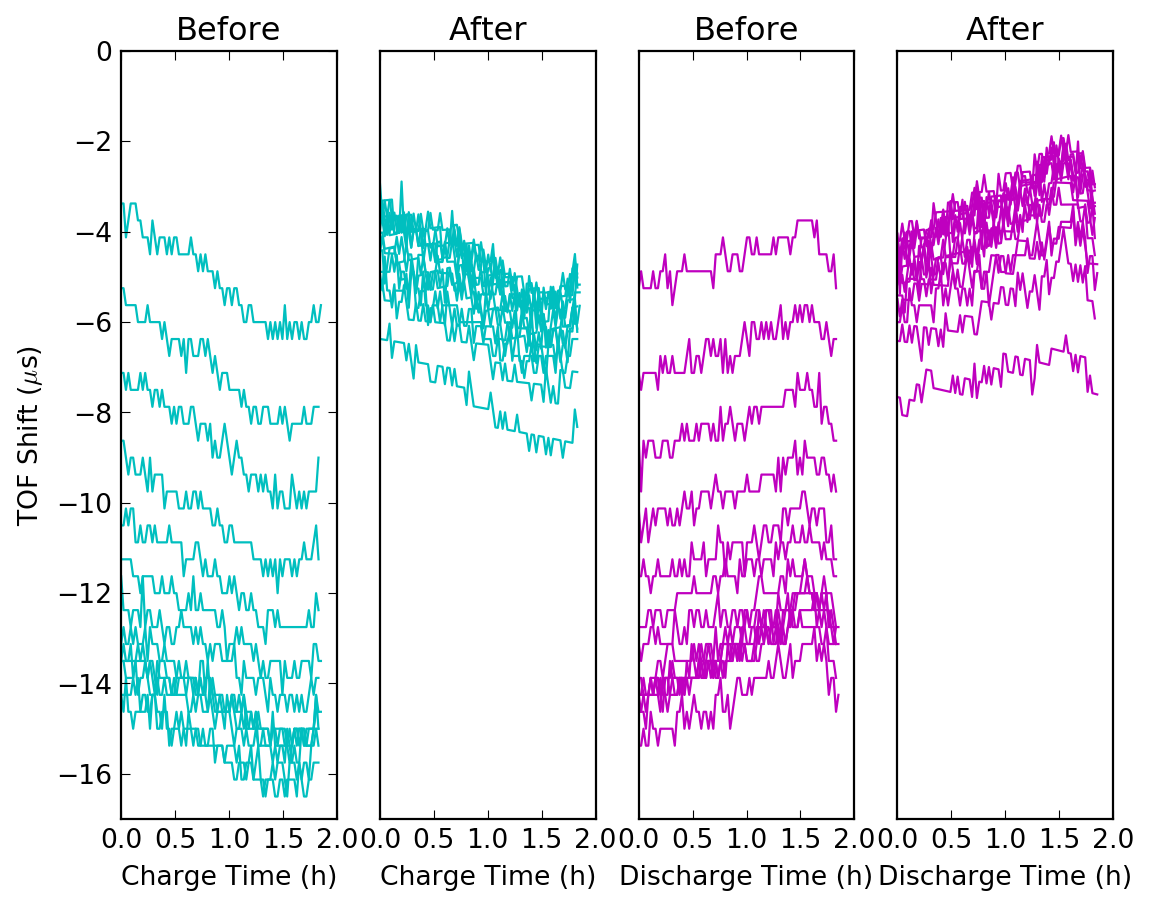
\includegraphics[width=0.95\textwidth]{Thesis/0417overlays.png}
\centering
\caption{Overlays of the raw and adjusted ToF shifts across each charge cycle (far and center left) and discharge cycle (center and far right). The adjusted data used a regression to remove the influence of ambient temperature fluctuations.}
\end{figure}


\chapter{Conclusion}

This thesis demonstrated the capability of acoustic time of flight analysis to observe changes in the state of charge and state of health in a fast-charge lithium-ion cell, and even to observe changes in the cell's ambient temperature. 

First, appropriate background was provided. Then, the requirements for and design of an experimental apparatus were provided. 
In short, this apparatus allows for the control of the three factors in shifts in time of flight of an acoustic wave through the lithium-ion cell: ambient conditions (in this case, temperature and pressure are of interest), cell state of charge, and cell state of health. 
The apparatus allows for the measurement and control of ambient temperature and pressure around the cell, and electrical load on the cell. 
Experimental procedures were established for observing and at times manipulating the electrochemical, acoustical, and thermal state of the cell and its environment. Finally, the data gathered while following those procedures was analyzed.

Ultimately, the analysis demonstrated the validity of acoustic time-of-flight analysis for observing changes in state of charge, state of health, and even ambient conditions in lithium-ion fast-charge cells. \todo{accomplished?} Further work could include going deeper into this line of research by building predictive models to quantify observed plating, developing an experimental apparatus and protocol that would allow for probing cells stacked in a more commercially-typical manner, or adapting the apparatus and analysis to work with cheaper, lower frequency sensors.

\bibliography{biblio}
\bibliographystyle{ieeetr}
\nocite{*}

%\appendix

%\chapter{An organ you don't need!}

But would sure like to have!

\end{document}